%% Introduction to latex facilities.
%% Sat 31 Dec 2005
%% Stephen Eglen.  
%% Text following a percent sign (%) until the end of line is treated
%% as a comment.

\documentclass[]{article}

%%%%%%%%%%%%%%%%%%%%%%%%%%%%%%%%%%%%%%%%%%%%%%%%%%%%%%%%%%%%%%%%%%%%%%
%% This section is called the preamble, where we can specify which
%% latex packages we required.  Most (but not of all) of the packages
%% below should be fairly standard in most latex documents.  The
%% exception is xspace and the new \latex command, which you probably
%% do not need.
%%%%%%%%%%%%%%%%%%%%%%%%%%%%%%%%%%%%%%%%%%%%%%%%%%%%%%%%%%%%%%%%%%%%%%

%% Bibliography style:
\usepackage{mathptmx}           % Use the Times font.
\usepackage{graphicx}           % Needed for including graphics.
\usepackage{url}                % Facility for activating URLs.
\usepackage{verbatim}           % For verbatiminput command.

%% Set the paper size to be A4, with a 2cm margin 
%% all around the page.
\usepackage[a4paper,margin=2cm]{geometry}

%% Natbib is a popular style for formatting references.
\usepackage{natbib}
%% bibpunct sets the punctuation used for formatting citations.
\bibpunct{(}{)}{;}{a}{,}{,}

%% This is an example of a new macro that I've created to save me
%% having to type \LaTeX each time.
\usepackage{xspace}
\providecommand*{\latex}{\LaTeX\xspace}

%%%%%%%%%%%%%%%%%%%%%%%%%%%%%%%%%%%%%%%%%%%%%%%%%%%%%%%%%%%%%%%%%%%%%%
%% Start of the document.
%%%%%%%%%%%%%%%%%%%%%%%%%%%%%%%%%%%%%%%%%%%%%%%%%%%%%%%%%%%%%%%%%%%%%%

\begin{document}

\author{Stephen J. Eglen\\
  Department of Applied Mathematics and Theoretical Physics\\
  University of Cambridge\\
  Wilberforce Road\\
  Cambridge CB3 0WA  U.K.}
\date{\today}
\title{A short example of how to use \latex in scientific reports}
\maketitle

\begin{abstract}
  The purpose of this short document is to provide a brief overview of
  the facilities that latex offers for formatting scientific reports.
  Furthermore, the source files for regenerating this report are
  freely available so that users can easily start writing their own
  reports using \latex.
\end{abstract}

\section{Introduction}

\latex is a typesetting program; given an input file with formatting
instructions (e.g intro.tex), the program will create your text
document in one of several formats (usually PDF, but also DVI and
Postscript).  It is therefore not a WYSIWYG word processor.  \latex is
known as a logical markup language, similar for example to HTML, so
that you describe a piece of text as a ``section heading'' rather than
saying that it should be formatted in a certain way.  It has excellent
facilities for typesetting mathematics, and handles large documents
(such as theses) well.  The aim of this document is not to provide an
overview of \latex, since many other guides have already been written
(see Section~\ref{sec:summary}).  Instead, it has been written
primarily to provide simple workable examples that you can cut and
paste to help you get started with \latex.  The examples have been
selected to be those most likely to be useful when writing a
scientific report.  This document is best read by comparing the source
code with the resulting output.

\section{Running \latex}

The files to accompany this paper are at:
\url{http://github.com/sje30/texintro}.  Get the
following files and put them into a new directory.

\begin{enumerate}
\item \url{intro.tex}: the main \latex document.
\item \url{example.bib}: a short bibliography.
%%\item \url{sigmoid.ps}: example postscript image.
\item \url{sigmoid.pdf}: example PDF image.
\end{enumerate}

Change directory to where you stored the files and type the
following (ignoring comments placed after \#\#):

\begin{verbatim}
pdflatex intro                  ## Run latex 1st time
bibtex intro                    ## Find references
pdflatex intro                  ## Run to resolve references
pdflatex intro                  ## sometimes twice!
xpdf intro.pdf                  ## View the resulting PDF
\end{verbatim}

You will notice that you run latex several times here; this is so that
references can be resolved, and references can be extracted from your
bibtex file.  After running latex, you will be told if you need to run
it again to resolve references.  After a while, you will get the hang
of how many times you need to run latex to resolve all your
references.  Or leave it to the machine/editor to do it for you with
tools like \textit{latexmk}.

\section{Tables}

Tables are relatively straightforward to generate.  Note that tables
and figures are not always placed exactly where you wish for them, as
they can \texttt{float} to other parts of the document.  Rather than
trying to battle with latex as to where they are placed, concentrate
first on getting the right content and let latex worry about the
positioning.  Instead, use labels to your tables to refer to them.
See Table~\ref{tab:simple} and Table~\ref{tab:pars} for examples.


\begin{table}
  \centering
  \begin{tabular}{|l|rr|}
    \hline
    year & min temp (C) & max temp (C)\\ \hline
    1970 & -5 & 35\\
    1975 & -7 & 29\\
    1980 & -3 & 30\\
    1985 & -2 & 32\\ \hline
  \end{tabular}
  \caption{Fictional minimal and maximal temperatures recorded in
    Cambridge over several years.}
  \label{tab:simple}
\end{table}

\begin{table}[htbp]
  \centering
  \begin{tabular}{lccc}\\ \hline
              & \multicolumn{1}{c}{$\phi$ (um)}
              & \multicolumn{1}{c}{$\alpha$}
              & $\delta_{12}$ (um)\\ \hline
    W81S1\\
    $h_{11}(u)$  & 67.94 & 7.81\\
    $h_{22}(u)$  & 66.27 & 5.40\\
    $h_{12}(u)$  &       &  &18\\
    \hline
    M623\\
    $h_{11}(u)$  &112.79 &  3.05\\
    $h_{22}(u)$  & 65.46 &  8.11\\
    $h_{12}(u)$        &&&20\\
        \hline
  \end{tabular}
  \caption{Summary of parameter estimates for the univariate
    functions $h_{11}(u)$, $h_{22}(u)$ and the bivariate function
    $h_{12}(u)$.  For the univariate fits, $\alpha$ and $\phi$ are 
    least-square estimates (assuming $\delta$ was fixed at 15 um).
    The final column gives the
    maximum likelihood estimate of $\delta_{12}$ assuming that the
    interaction between types is simple inhibition.
    \label{tab:pars}}
\end{table}

\section{Bibliography management}

Scientific reports normally require a references section where your
references are cited.  Bibtex is an excellent system for maintaining
references, especially for large documents.  Each reference needs a
unique key; you can then refer to the reference in your \latex
document by using this key within a cite command.

Take care when formatting your references, especially when it comes to
writing authors names and the case of letters in journal titles.  In
our examples, the references are found in \url{example.bib}.  As an example
of a citation, see \citep{ihaka1996} or \citep{ihaka1996,venables1999}.

Bibtex is flexible enough to format your references in a wide number
of different styles to suit your needs.  In this file I have used the
``natbib'' package, which is suitable for the Natural Sciences.
Depending on the type of cite command you get (and the package that
you use for citations), you can get different styles of citation.  See
Table~\ref{tab:cite} for some examples.

\begin{table}
  \centering
  \begin{tabular}{ll}
    \hline
    command & result\\ \hline
    \verb+\citep{ihaka1996}+ & \citep{ihaka1996}\\
    \verb+\citet{ihaka1996}+ & \citet{ihaka1996}\\
    \verb+\citep[see][p. 300]{ihaka1996}+ &
    \citep[see][p. 300]{ihaka1996}
    \\
    \verb+\citeauthor{ihaka1996}+ & \citeauthor{ihaka1996}
    \\
    \verb+\citeyear{ihaka1996}+ & \citeyear{ihaka1996}
    \\
    \hline
  \end{tabular}
  \caption{Examples of different citation commands available in the
    natbib package.}
  \label{tab:cite}
\end{table}

\section{Graphics} \label{sec:graphics}

Create your images for pdflatex as either pdf (preferred for vector
formats), png or jpeg.  Figures can be included either at their
natural size, or you can specify e.g. how wide you wish the figure to
be. Figure~\ref{fig:example} shows an example image which
intentionally looks slightly different depending on whether you
compile the document with latex or pdflatex.  Note that in this
example the suffix of the image file is not included, in which case
pdflatex will look for a file with a supported suffix.

\begin{figure}
  \centering
  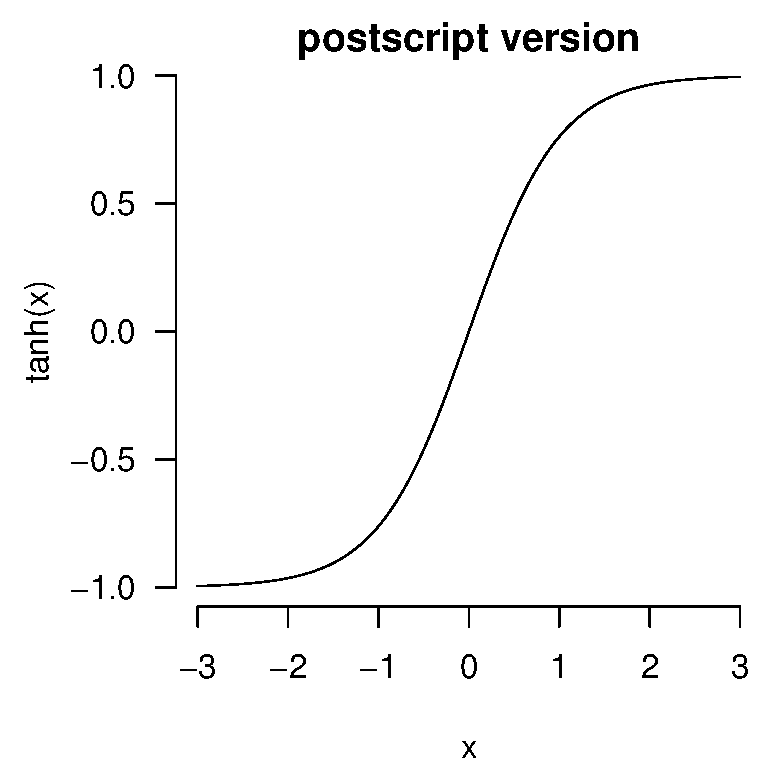
\includegraphics[width=6cm]{sigmoid}
  \caption{Example of a sigmoidal curve generated by the R programming
    environment.  The title above the curve indicates whether you have
  included the postscript or the pdf version of the figure.}
  \label{fig:example}
\end{figure}

\section{Mathematics}

\latex can format mathematics with ease, either in line, such as 
$x \times y$, or on separate lines, such as:

\[ x^2 +y^2 = z^2 \]

If you are writing several lines of equations, you can use statements
like the following:

\begin{eqnarray}
  b(t) & = & s(t) - \int_{0}^{T} a(t') \cdot i(T-t') dt'
  \\
  a(t) & = & \int_{0}^{T} b(t) \cdot e(T-t') dt' \label{eq:am}
  \\
  g(t) & = & b(t) \ast e(t) \nonumber
\end{eqnarray}

By using labels on certain equations, we can refer to equations by
number, such as equation~(\ref{eq:am}).

\section{Including text ``as-is''}

In your reports you may wish to sometimes include text ``as-is'', with
no subsequent markup from \latex.  There are several ways to achieve
this, using verbatim commands.  For example \verb+longest_word = 99+
is verbatim text, as is the following paragraph:

\begin{verbatim}
one two three
four five
six
\end{verbatim}

See the \textit{listings} package for sophisticated ways of formatting
code written in different computing languages.  Finally, if you would
like to include the contents of a file, use \verb+\verbatiminput+from
the \textit{verbatim} package, as used here to list our bibtex
references:

\subsection{Contents of bibliography}

\verbatiminput{example.bib}

\section{Summary}
\label{sec:summary}
This short guide should give you a flavour of what can be done with
\latex.  It is by no means complete, or supposed to be
self-explanatory.  It is, however, hopefully enough to get you
started!  Try experimenting by editing the source file and then
recompiling this document.  As mentioned earlier, there are many
guides for latex.  Two that I can recommend are
\url{http://www.andy-roberts.net/misc/latex/index.html} and 
`` The (Not So) Short Introduction to LaTeX2e''
(\url{http://ctan.tug.org/tex-archive/info/lshort/english/lshort.pdf}).

%%%%%%%%%%%%%%%%%%%%%%%%%%%%%%%%%%%%%%%%%%%%%%%%%%%%%%%%%%%%%%%%%%%%%%
%% Finally we specify the format required for our references and the
%% name of the bibtex file where our references should be taken from.
%%%%%%%%%%%%%%%%%%%%%%%%%%%%%%%%%%%%%%%%%%%%%%%%%%%%%%%%%%%%%%%%%%%%%%

\bibliographystyle{plainnat}
\bibliography{example}

\end{document}

%%%%%%%%%%%%%%%%%%%%%%%%%%%%%%%%%%%%%%%%%%%%%%%%%%%%%%%%%%%%%%%%%%%%%%
%% The end.
%%%%%%%%%%%%%%%%%%%%%%%%%%%%%%%%%%%%%%%%%%%%%%%%%%%%%%%%%%%%%%%%%%%%%%